\chapter{Praktische Evaluation}

\section{Testumgebung}
Die folgenden Experimente wurden auf mithilfe einer AMD EPYC 7763 64-Core CPU mit 16 nutzbaren Hardwarethreads und 64GB Arbeitsspeicher durchgeführt. Das System
verwendet Ubuntu 24.04 als Betriebssystem und GCC in der Version 13.2.0 als Compiler. Die Ausführung der Algorithmen mit einer spezifischen Anzahl von Threads wurde
softwareseitig über OpenMP-Instruktionen realisiert. 

\section{Implementierung}

\subsection{Klassenstruktur}
\begin{figure}[ht]
    \centering
    \caption{Klassenstruktur der Implementierung}
    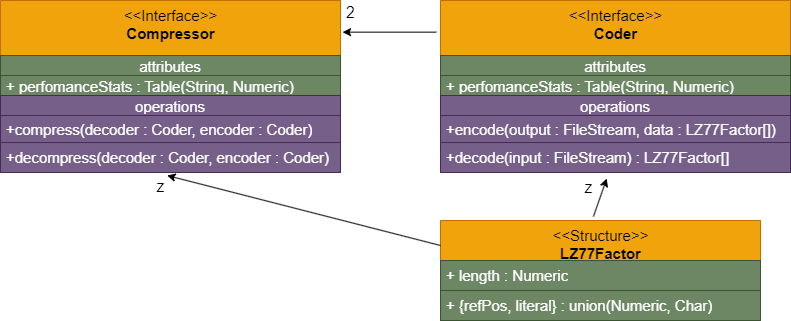
\includegraphics[scale=0.4]{Images/uml.png} \label{uml}
\end{figure}

Die in \ref{uml} dargestellte Klassenstruktur illustriert die grundlegende Abstraktion, die für die Implementierung der Algorithmen verwendet wurde. Compressor und
Coder beschreiben jeweils ein Interface bzw. ein Template, welches durch ein konkretes Kompressionsverfahren und einer Kodierung spezialisiert werden kann. Jegliche
Spezialisierungen teilen sich jedoch eine gemeinsame Definition eines Faktors im LZ77-Schema.

\subsection{Externe Bibliotheken}
Im Folgenden werden die genutzten externen Bibliotheken aufgelistet, die im Rahmen der Implementierung der Algorithmen, sowie deren Evaluation genutzt wurden.
\subsubsection{Malloc Count}
Malloc Count\cite{malloc_count} ist eine C++-Bibliothek, die es ermöglicht, Speicherallokationen und -freigaben auf dem Heap zu überwachen und zu messen. Im
Rahmen unserer Evaluation gibt uns diese Bibliothek die Spitze des allokierten Speichers innerhalb des Ausführung der Algorithmen aus.

\subsubsection{Unordered-Dense-Map}
Die Unordered-Dense-Map\cite{unordered_dense} stellt eine hochperformante Hashtabelle dar, die insbesondere in der Dauer ihrer Suchoperationen gegenüber
der std::unordered\_map aus der Standardbibliothek deutlich trumpft. Dies Hashtabelle wurde in Approx.LZ77 und Approx.LZ77Par für die Speicherung der
RFPs in jeder Runde verwendet. Im Rahmen der Entwicklung von Approx.LZ77Par hat sich die Verwendung mehrerer Instanzen von Unordered-Dense-Map im Vergleich
zu anderen inherent parallelen Hashtabellen\cite{oneapi}\cite{sharded_map} als effizienter herausgestellt.

\subsubsection{LibSaiS}
Für die Implementierung der exakten LZ77-Faktorisierung, die als Referenzalgorithmus fungiert, wurde die Bibliothek LibSaiS\cite{libsais} zu Hilfe genommen. Diese
Bibliothek stellt eine effiziente Implementierung für die Konstruktion des Suffix-Arrays bereit.

\section{Messung}

\subsection{Eingabedaten}
Die folgenden Algorithmen wurden auf verschiedenen Dateien aus dem Pizza \& Chili-Corpus getestet. Die verwendeten Dateien decken verschiedene Kontexte und damit
Kompressionspotentiale ab.
\begin{figure}[ht]
    \centering
    \caption{Auflistung der verwendeten Eingabedaten}
    \label{inputdata}
    \begin{tabular}{|c|c|c|c|c|}
        \hline
        \textbf{Datei} & \textbf{Größe} & \textbf{Alphabetgröße} & \textbf{Beschreibung} \\
        \hline
        \texttt{dna} & 200MB & 4 & DNA-Sequenzen \\
        \hline
        \texttt{english} & 200MB & 256 & Englische Texte \\
        \hline
        \texttt{proteins} & 200MB & 20 & Proteinsequenzen \\
        \hline
        \texttt{sources} & 200MB & 256 & Quellcode \\
        \hline
        \texttt{xml} & 200MB & 256 & XML-Dateien \\
        \hline
    \end{tabular}
\end{figure}
In der Tabelle \ref{inputdata} sind die verwendeten Dateien aufgelistet. Die Größe der Dateien wurde auf 100MB beschränkt, um einen angemessenen Rahmen für die 
Laufzeitmessung zu erhalten.

\subsection{Messgrößen}

\subsubsection{Laufzeit}
Die Laufzeit der Algorithmen wurde innerhalb der Ausführung gemessen. Dabei wird die Zeitmessung nach dem Laden der Eingabedatei gestartet und mit dem vollständigen
Auffüllen der Faktorfolge beendet. Damit wird das Einlesen der Eingabe und eine eventuelle Kodierung der Ausgabe nicht in die Laufzeitmessung einbezogen. Diese Strategie
hat ihren Hintergrund in der Tatsache, dass die konkrete Ausprägung des Eingabe- und Ausgabestroms keine Aussagekraft über die Qualität der Kompression hat.

\subsubsection{Speicher}
Der Speicherverbrauch der Algorithmen wurde auch intern mithilfe einer externen Bibliothek gemessen. Dabei wurden Speicherallokationen auf dem Heap überwacht und 
gemessen. Im Rahmen dieser Arbeit wurde die Spitze des allokierten Speichers im Zeitraum nach dem Einlesen der Eingabedatei und nach dem vollständigen Auffüllen der
Faktorfolge gemessen.

\subsubsection{Kompressionsrate CR*} \label{cr}
Die Kompressionsrate wird neben der Anzahl der Faktoren zum Großteil von der verwendeten Kodierung bestimmt. Wie bereits erwähnt, sind wir in der Wahl der Kodierung
nicht beschränkt, sodass die Aussagekraft bezüglich der Qualität der Kompression nicht eingeschränkt ist. Es ist jedoch zu beachten, dass Faktoren, die durch Approx. LZ77
erzeugt werden stets eine Zweierpotenz als Länge annehmen. Die binäre Repräsentation dieser Längen kann daher in Abhängigkeit von der gewählten Kodierung kompakt 
konstruiert werden. Um dieses Phänomen zu illustrieren gehen wir im Folgenden eine naive Kodierung vor, auf dessen Grundlage wir die Kompressionrate $CR*$ definieren.
\begin{equation}
    |K_{LZ77}(f)| = 1 + \begin{cases}
        2\log_2(n) & \text{falls } |f| > 1 \\
        9 & \text{sonst}
    \end{cases}
\end{equation}
Im Falle von LZ77 bestimmt ein Bit, ob es sich um eine Referenz oder ein einzelnes Zeichen handelt. Im Falle einer Referenz wird die Länge und die Position der Referenz
mithilfe von $\log_2(n)$ Bits kodiert. Im Falle eines einzelnen Zeichens wird die ASCII-Kodierung des Zeichens verwendet, die 8 Bits benötigt.
\begin{equation}
    |K_{Approx.LZ77}|= 1 + \begin{cases}
        \log_2(n)+\log_2(\log_2(n)) & \text{falls } |f| > 1 \\
        9 & \text{sonst}
    \end{cases}
\end{equation}
Im Falle von Approx. LZ77 kann die Länge mithilfe von $\log_2(\log_2(n))$ Bits kodiert werden, da die Länge anhand einer einzelnen Bitposition bestimmt wird.

\newpage
\subsection{Messwerte}

\begin{table}[ht]
    \centering
    \caption{Messgrößen der Algorithmen}
    \label{messwerte}
    \begin{tabular} { |c|c|c|c|c|c| }
        \hline
        \textbf{Eingabe} & \textbf{Algorithmus} & \textbf{Laufzeit[s]} & \textbf{Speicher[Byte]} & \textbf{FR} & \textbf{CR*} \\
        \hline
        & LZ77 & 15.40 & 20.00 & 9.98\% & 70.83\% \\
        proteins & Approx.LZ77 & 44.06 & 9.94 & 15.34\% & 63.95\% \\
        & Approx.LZ77Par & 6.99 & 10.21 & 15.34\% & 63.95\% \\
        \hline
        & LZ77 & 13.47 & 20.00 & 5.60\% & 38.75\% \\
        sources & Approx.LZ77 & 40.43 & 6.42 & 10.05\% & 40.14\% \\
        & Approx.LZ77Par & 6.49 & 5.90 & 10.05\% & 40.14\% \\
        \hline
        & LZ77 & 15.36 & 20.00 & 6.70\% & 47.24\% \\
        english & Approx.LZ77 & 51.00 & 7.06 & 10.42\% & 43.39\% \\
        & Approx.LZ77Par & 7.46 & 6.16 & 10.42\% & 43.39\% \\
        \hline
        & LZ77 & 14.89 & 20.00 & 6.66\% & 47.46\% \\
        dna & Approx.LZ77 & 30.10 & 8.38 & 10.71\% & 45.53\% \\
        & Approx.LZ77Par & 4.80 & 6.66 & 10.71\% & 45.53\% \\
        \hline
        & LZ77 & 13.02 & 20.00 & 3.42\% & 23.61\% \\
        xml & Approx.LZ77 & 29.38 & 3.46 & 6.62\% & 26.78\% \\
        & Approx.LZ77Par & 4.91 & 3.46 & 6.62\% & 26.78\% \\
        \hline
    \end{tabular}
\end{table}

\subsubsection{Laufzeiten}
\begin{figure}[ht]
    \centering
    \caption{Laufzeitmessung von LZ77, Approx.LZ77 und Approx.LZ77Par(16 Threads) auf verschiedenen Präfixen von proteins. Als Vergleichsmaß wurde 
    die lineare Regression der Kurven gestrichelt eingezeichnet.}
    \label{runtime}
    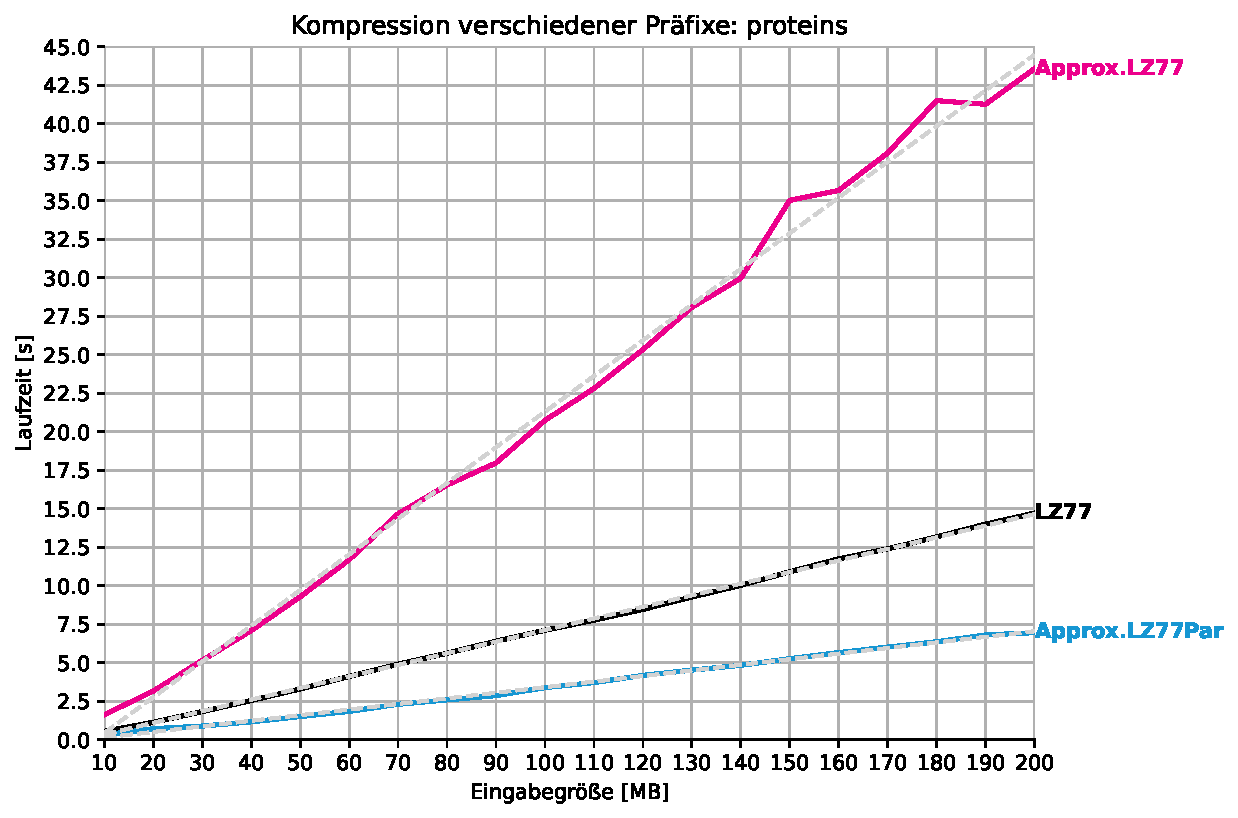
\includegraphics[scale=0.6]{Images/progressive_proteins.pdf}
\end{figure}
    
\begin{figure}[ht]
    \centering
    \caption{Laufzeitmessung von Approx.LZ77Par mit verschiedener Anzahl an Threads für proteins}
    \label{runtime_threads}
    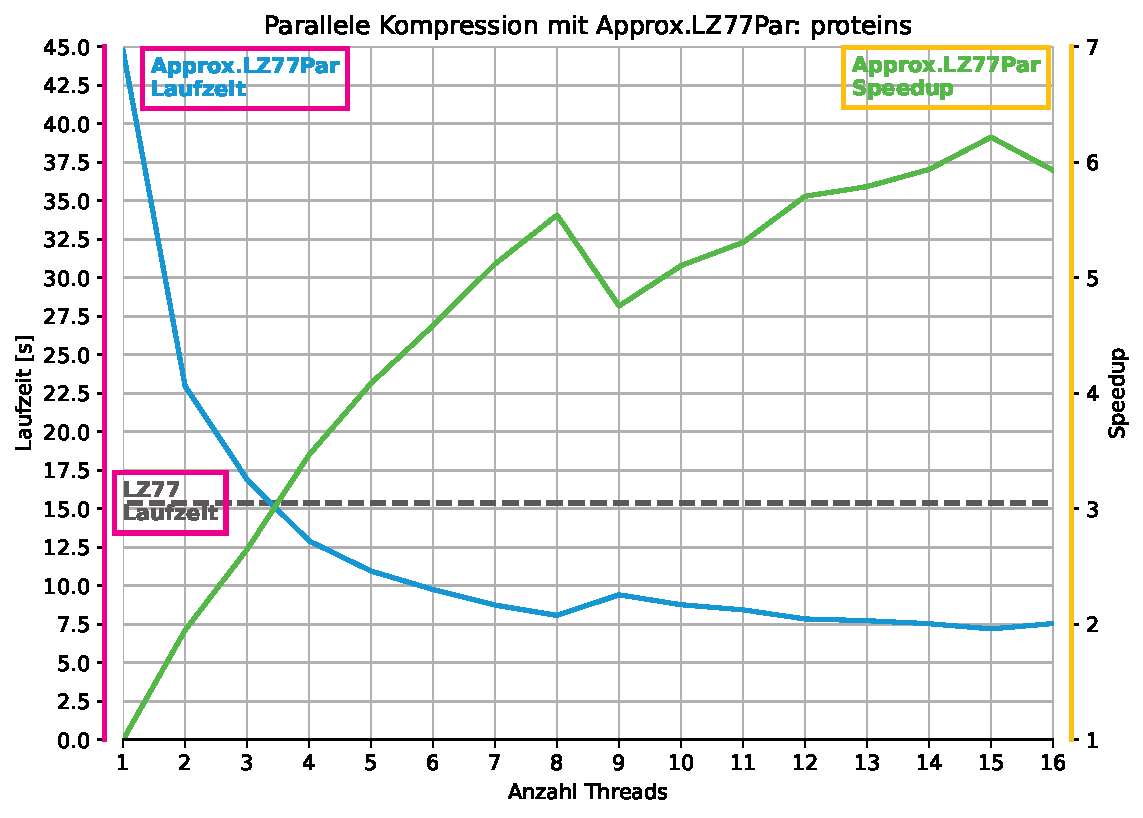
\includegraphics[scale=0.6]{Images/progressive_speedup_proteins.pdf}
\end{figure}

\subsubsection{Speicherverbrauch}
\begin{figure}[ht]
    \centering
    \caption{Speicherverbrauch von LZ77, Approx.LZ77 und Approx.LZ77Par(16 Threads) auf verschiedenen Präfixen von proteins. Aufgezeichnet wurde das Verhältnis
    von allokiertem Speicher zur Eingabegröße.}
    \label{memory}
    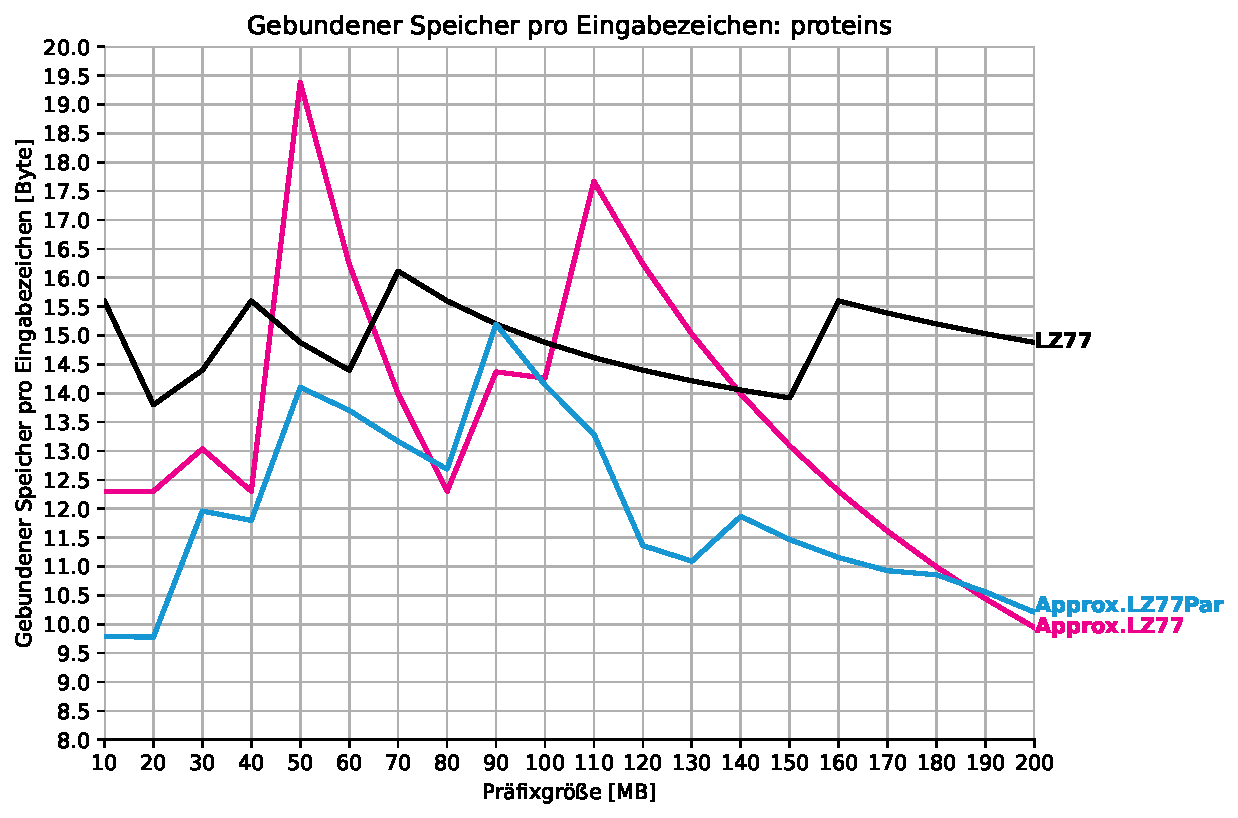
\includegraphics[scale=0.6]{Images/progressive_mem.pdf}
\end{figure}
\subsubsection{FR und CR*}

\section{Auswertung}
\subsection{LZ77}
Wie in Kapitel 3.1 beschrieben, zeigt der verwendete Algorithmus zur Generierung einer exakten LZ77-Faktorisierung ein lineares Verhalten bezüglich der Laufzeit.
Dies wird in Abbildung \ref{runtime} deutlich, wo die Laufzeitmessung von LZ77 auf verschiedenen Präfixen von proteins dargestellt ist. Die lineare Regression der
Kurven verdeutlicht das lineare Verhalten. Auch im Bezug auf die Speichernutzung wird das lineare Verhältnis zur Eingabegröße in Abbildung \ref{memory} deutlich.
Das Verhältnis von allokiertem Speicher zur Eingabegröße beträgt in nahezu allen Präfixen von proteins 20 Byte pro Eingabezeichen. Hiermit konnten wir die theoretische
Analyse des Laufzeit- und Speicherverhaltens empirisch bestätigen.

\subsection{Approx. LZ77}
In \ref{messwerte} wird deutlich, dass Approx. LZ77 dem exakten LZ77-Algorithmus in der Laufzeit und der Faktorrate stets deutlich unterlegen ist. Wie bereits in Kapitel
3.2 beschrieben, liegt der Fokus von Approx. LZ77 auf der Reduktion des Speicherverbrauchs. Weiterhin wurde eine schlechtere theoretische Laufzeitkomplexität von
$O(n\log n)$ gegenüber $O(n)$ für LZ77 festgestellt. Die Messwerte in \ref{messwerte} bestätigen diese theoretische Analyse damit. Es ist jedoch zu beachten, dass
Approx. LZ77 wie zu erwarten auch eine deutlich bessere Speichernutzung aufweist, wobei diese stark von der Eingabe abhängt. In Abbildung \ref{memory} wird deutlich, dass
selbst verschiedene Präfixe einer Eingabedatei unterschiedliche relative Speichernutzungen aufweisen. Dies lässt sich auf ein unterschiedliches Maß der Redundanz in den
Eingaben zurückführen. Die Kompressionsrate $CR*$ von Approx. LZ77 ist in \ref{messwerte} ebenfalls aufgeführt. Es ist zu erkennen, dass die Abweichung der Kompressionsrate
von LZ77 in den meisten Fällen geringer ausfällt als die Abweichung der Faktorrate. Dies ist auf die in \ref{cr} beschriebene Eigenart der Kodierung zurückzuführen.

\subsection{Approx. LZ77Par}
Im Bezug auf die Qualität der Kompression weist die Approx.LZ77Par keine Unterschiede zu Approx.LZ77 auf, was als Indiz für die Korrektheit der Implementierung
interpretiert werden kann. Die Laufzeitmessung in \ref{runtime} zeigt, dass Approx.LZ77Par mit 16 Threads eine deutlich bessere Laufzeit aufweist als Approx.LZ77.
Die Laufzeitmessung in \ref{runtime_threads} zeigt, dass die Laufzeit von Approx.LZ77Par von einer kleinen Anzahl an Threads stärker profitiert. Mit zunehmender 
Anzahl an Threads wird die Beschleunigung bzw. der Speedup geringer. Die resultierende Asymptote in der Laufzeitmessung ist auf externe Faktoren zurückzuführen,
wie der Bandbreite der Speicherzugriffe und Symptomen von False Sharing. Der Speicherverbrauch von Approx.LZ77Par ist in \ref{memory} ebenfalls aufgezeichnet.
Es fällt auf, dass der Speicherverbrauch von Approx.LZ77Par im Vergleich zu Approx.LZ77 in den meisten Fällen leicht geringer ausfällt. 
Dies ist auf die Verwendung von mehreren Instanzen von Unordered-Dense-Map zurückzuführen, die aufgrund ihrer inhärenten Struktur einen geringen gesamten
Speicherverbrauch aufweisen. 